\section{Research Questions, Methodology, and Implementation}


In light of the results of the previous works, we aim to investigate the following research questions through a large-scale study of Greek and UK domains: 

\begin{enumerate}[label=\textbf{RQ\arabic*}:, ref=RQ\arabic*, leftmargin=1.05cm]
    \item \label{rq:prevalence} What is the prevalence of cookie banners across the board when less popular websites in Greece and the UK are also considered? 
    \item \label{rq:avg_options} How does the distribution of options offered in cookie banners look like and what proportion of websites provide a direct cookie rejection option?
    \item \label{rq:no_options} What proportion of websites employ implicit consent?
    \item \label{rq:manage_options_count} What proportion of cookie banners allows their users to manage their privacy settings and control which vendors track them?
    \item \label{rq:distribution} How do the countries compare in terms of the privacy options offered by cookie banners? 
\end{enumerate}

Our data collection included three steps. We first built a comprehensive set of functioning websites to analyse and extract their cookie banners. Then we crawled the identified websites and collected relevant data such as the source code of the cookie notices and screenshots of the webpages. Finally, we sanitised and structured the collected data into a data structure that facilitates analysis. 
In the following, we explain these steps in more detail. 
The code developed for this study and referred to throughout the paper is publicly available at the following repository: \url{https://github.com/kampanosg/i-like-cookies}. 

\subsection{Building the Target List}
The first step is to identify websites to be analysed in this study. Using the Tranco top sites ranking~\cite{LePochat2019}, popular websites for the two countries were identified based on their Top Level Domains (TLDs): \texttt{.uk} and \texttt{.gr}. 
We decided to augment the TLD-based lists with other curated country-specific lists since many websites do not use the TLD of their country of origin, e.g.,  British Airways uses \texttt{.com}. 

\paragraph{Ethical Considerations.}
Not all websites allow crawling and many explicitly state that they only allow \say{personal use} of their services and content to their visitors. To respect such restrictions imposed by the websites, we developed two parsers to identify and exclude such websites from our automated crawl: 

\begin{enumerate}
    \item A Robots Exclusion Standard parser (\texttt{step1b\_checker\_robots.py}) that verifies whether websites allow crawling by reading their \texttt{robots.txt} file;
    
    \item A Terms of Service (ToS) parser (\texttt{step1c\_checker\_tos.py}) that makes best effort to find exclusionary terms, e.g. \say{for personal use only}, to comply with the ToS of each website.
\end{enumerate}

\subsection{Collecting Cookie Banners}
The second step is to effectively identify and collect the cookie banners on the compiled set of websites. We achieve this by taking advantage of the \say{I don’t care about cookies} (IDCAC) list (\url{www.i-dont-care-about-cookies.eu}), which provides an extensive selection of standard CSS selectors that cookie banners use. We parse these selectors and add them to a database. Furthermore, during testing, we identified and added 64 additional selectors to IDCAC.

After setting up the cookie selectors database, OpenWPM uses it to identify the cookie banners within the visited websites. We extended OpenWPM to detect cookie banners within a given website. For each website, we check whether it contains a CSS selector from the cached IDCAC list, using Selenium (\url{www.selenium.dev}), which allows for searching the HTML code of the website. When OpenWPM identifies a cookie banner, we perform additional analysis to make sure it is not a false positive, briefly by first ensuring that Selenium returned a valid HTML of a reasonable length, and then verifying that the returned HTML contains the terms \say{cookie} or \say{cookies}. 

When OpenWPM successfully identifies a cookie banner, it is stored in a database for further analysis. Combining the cached cookie selectors and Selenium's efficient Document Object Model (DOM) search enables the cookie banner extension to be efficient and robust. 

\subsection{Classifying and Normalising the Data}
To our knowledge, no standard exists for cookie banners, and therefore, every website has a different implementation for their notices. Thus, the HTML code and the options they provide can be drastically different from website to website. Such complexity can make the data analysis difficult. Thus, before performing any research on the data, we transformed them into a consistent data structure. 

\begin{table}[t]
    \centering
    \caption{The developed cookie banner options categories.}
    \begin{tabular}{@{}l@{\quad}l@{}}
    \toprule
        \textbf{Category} & \textbf{Description}                                   \\ \midrule
        Affirmative     & Options that prompt users to accept the use of cookies, \\
                        & e.g. \say{accept}, \say{agree}, \say{allow}, and \say{OK}.                                  \\
        Negative        & Options that allow users to opt-out from cookie tracking,        \\ 
                        & e.g. \say{decline}, \say{reject}, \say{disagree}, and \say{no}.                            \\
        Informational   & Options that take users to informational pages, e.g. \\
                        & \say{Privacy Policy}, \say{learn/see more}, and \say{see/show details}.                               \\
        Managerial      & Options that allow users to opt in/out of specific trackers,  \\ 
                        & e.g. \say{manage}, \say{settings}, and \say{vendors/partners}.                     \\ \bottomrule
    \end{tabular}
    \label{tab:privacy_options_categories}
\end{table}

First, we sanitised the collected data to identify and then classify the privacy options within the collected cookie banners. We identified four privacy option categories: \emph{Affirmative}, \emph{Negative}, \emph{Informational} and \emph{Managerial} as defined in Table \ref{tab:privacy_options_categories}. We developed these four categories by manually inspecting a random sample of the collected data during testing, further informed by our own experience with cookie banners in the wild. Using these categories allows us to classify the cookie banners by the types of options they provide and hence better understand user choices. Examples of cookie banners providing different combinations of these options can be seen in Fig.~\ref{fig:cookie_banners}. 


\begin{figure}[t]
    \centering
    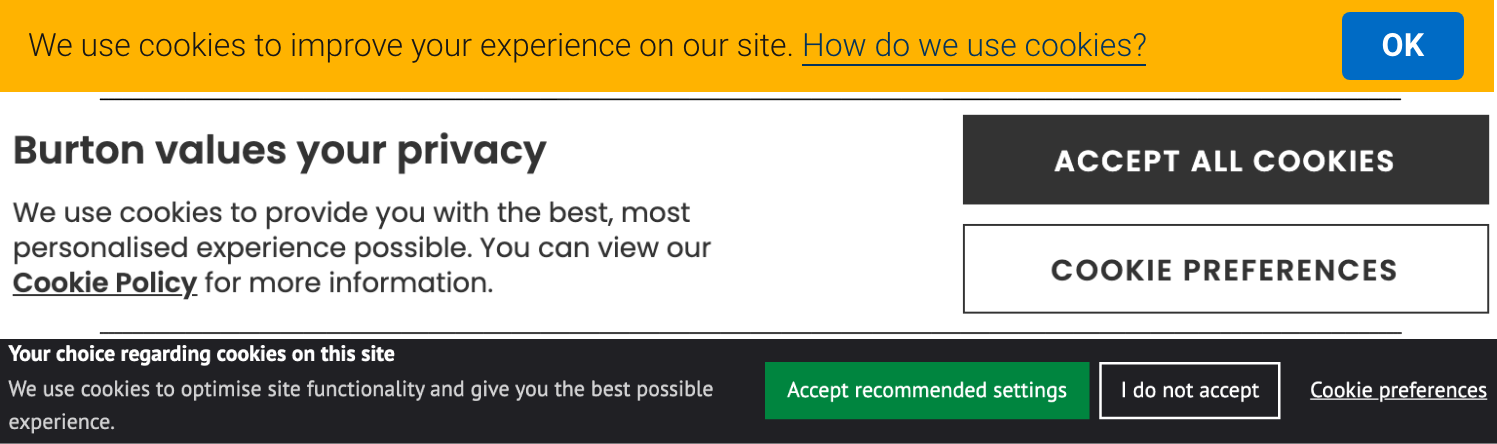
\includegraphics[width=\textwidth]{images/methodology/cookie_banners.png}
    \caption{Three examples of cookie banners with different privacy options. 
             Top: Affirmative and Informational, 
             Middle: Affirmative, Managerial, and Informational, 
             Bottom: Affirmative, Negative, and Managerial.}
    \label{fig:cookie_banners}
\end{figure}

Manual inspection of the privacy options was necessary to account for local nuances. For example, although the noun $\alpha\pi o\delta o\chi\eta$ (lit. acceptance) was the most popular Affirmative call to action, a large number of banners used the verb $\delta\epsilon\chi o\mu\alpha\iota$ (I accept) indicating the same. We developed a comprehensive list of such variations and wrote a Python script (\texttt{step3a\_parse\_cookie\_banners.py}) to categorise cookie banners.

After we categorised the privacy options, we transformed the collected data into a consistent data structure that allows for efficient querying. More specifically, we converted the arbitrary HTML form of the collected cookie notices into JSON to facilitate both manual and automated analyses. 

Fig.~\ref{fig:html2json} depicts an example banner before and after categorisation and normalisation.


\begin{figure}[t]
    \centering
    \begin{lstlisting}[language=HTML, style=lst_style]
    <div class="..." aria-hidden="true" data-contents="...">
     <div class="container">
      <p class="...">By visiting x.gr you agree to the use of cookies.</p>
      <a href="#" class="...">Agree</a>
     </div>
    </div>
    \end{lstlisting}
    \begin{lstlisting}[language=json, style=lst_style]
    {
     "has_accept_btn": 1, 
     "accept-btn_cta": "Accept", 
     "privacy_text": "By visiting x.gr you agree to the use of cookies.", 
     ... 
    }
    \end{lstlisting}
    \caption{A cookie banner before (top) and after (bottom) normalisation}
    \label{fig:html2json}
\end{figure}